\documentclass[standalone, border=10pt]{standalone}
\usepackage{pgfplots}
\pgfplotsset{compat=1.17}

\begin{document}

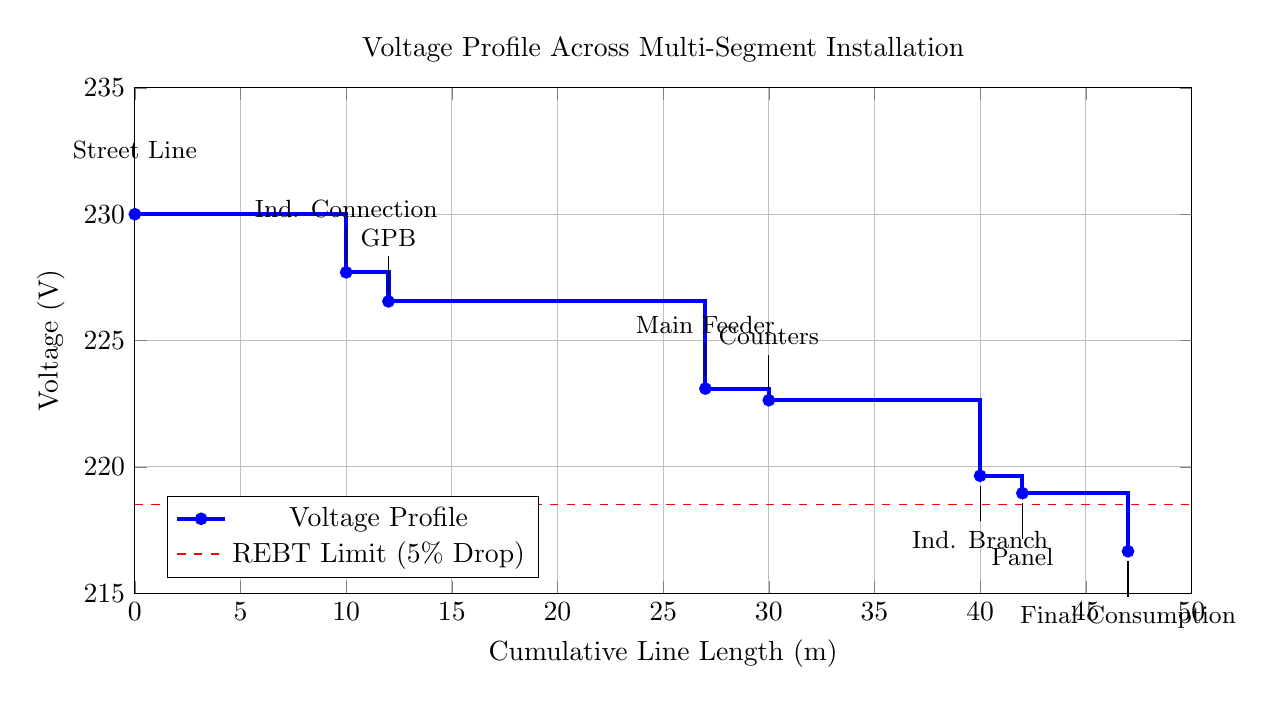
\begin{tikzpicture}
    \begin{axis}[
        title={Voltage Profile Across Multi-Segment Installation},
        xlabel={Cumulative Line Length (m)},
        ylabel={Voltage (V)},
        width=15cm, 
        height=8cm,
        grid=major,
        legend pos=south west,
        xmin=0,
        xmax=50,
        ymin=215,
        ymax=235,
    ]
    
    % The plot with new, detailed coordinates for each stage
    \addplot[const plot, blue, line width=1.5pt, mark=*, mark size=1.5pt] coordinates {
        (0, 230)      % Start
        (10, 227.7)   % Drop 1.0%
        (12, 226.55)  % Drop 0.5%
        (27, 223.1)   % Drop 1.5%
        (30, 222.64)  % Drop 0.2%
        (40, 219.65)  % Drop 1.3%
        (42, 218.96)  % Drop 0.3%
        (47, 216.66)  % Drop 1.0%
    };
    \addlegendentry{Voltage Profile}
    
    % The 5% voltage drop limit line
    \addplot[dashed, color=red] coordinates {(0, 218.5) (50, 218.5)};
    \addlegendentry{REBT Limit (5\% Drop)}

    % Define coordinates for the pin labels
    \coordinate (p0) at (axis cs:0, 230);
    \coordinate (p1) at (axis cs:10, 227.7);
    \coordinate (p2) at (axis cs:12, 226.55);
    \coordinate (p3) at (axis cs:27, 223.1);
    \coordinate (p4) at (axis cs:30, 222.64);
    \coordinate (p5) at (axis cs:40, 219.65);
    \coordinate (p6) at (axis cs:42, 218.96);
    \coordinate (p7) at (axis cs:47, 216.66);
    
    \end{axis}
    
    % Add annotations using pins attached to the coordinates.
    % Placed outside the 'axis' environment to prevent clipping.
    \node[pin={[pin edge={black, thin}, text=black, font=\small]90:{Street Line}}] at (p0) {};
    \node[pin={[pin edge={black, thin}, text=black, font=\small]90:{Ind. Connection}}] at (p1) {};
    \node[pin={[pin edge={black, thin}, text=black, font=\small]90:{GPB}}] at (p2) {};
    \node[pin={[pin edge={black, thin}, text=black, font=\small]90:{Main Feeder}}] at (p3) {};
    \node[pin={[pin edge={black, thin}, text=black, font=\small]90:{Counters}}] at (p4) {};
    \node[pin={[pin edge={black, thin}, text=black, font=\small]-90:{Ind. Branch}}] at (p5) {};
    \node[pin={[pin edge={black, thin}, text=black, font=\small]-90:{Panel}}] at (p6) {};
    \node[pin={[pin edge={black, thin}, text=black, font=\small]-90:{Final Consumption}}] at (p7) {};
    
\end{tikzpicture}

\end{document}

